\documentclass[12pt]{article} 
\usepackage[russian]{babel}
\usepackage{amsmath}			% for math formulas
\usepackage{amsthm}
\usepackage{setspace}
\usepackage{amsfonts}			% for math formulas
\usepackage{amssymb}
\usepackage[unicode, pdftex]{hyperref}
\usepackage[left=25mm, top=20mm, right=25mm, bottom=20mm, nohead, nofoot]{geometry}
\usepackage{graphicx}
\pagestyle{empty}

\begin{document}

%-------------------------------
%	TITLE SECTION
%-------------------------------


\begin{flushleft}
\url{https://www.facebook.com/profile.php?id=10000654912}
\url{https://github.com/lovgager/latex}
\end{flushleft}
\hrule 
\begin{flushright}
16.04.2021
\end{flushright}
\bigskip

%-------------------------------
%	CONTENTS
%-------------------------------

\newtheorem*{task}{Задача}
\begin{task}
Вычислить
\begin{equation}\label{integral}
    I = \int\limits_0^{16\sqrt[4]{\pi}} x\,dx \int\limits_{x^2/256}^{\sqrt{\pi}} \sin{y^2}\;dy.
\end{equation}
\end{task}

\noindent\textbf{Решение.} Внутренний интеграл вычислить не получается, поскольку он представляет собой неберущийся интеграл Френеля: первообразная от $f(y)=\sin{y^2}$ не выражается через элементарные функции. Попробуем изменить порядок интегрирования, зная, что ответ останется тем же. Для этого следует изобразить область на плоскости переменных $x,y$ согласно значениям, стоящим в пределах интегралов. Переменная $x$ может принимать значения от $0$ до $\sqrt[4]{\pi}$, а $y$ меняется в зависимости от значения $x$, а именно от $x^2/256$ до $\sqrt{\pi}$. Область интегрирования $S$ представляет собой фигуру, ограниченную двумя прямыми линиями и дугой параболы, как на рисунке:
\begin{center}
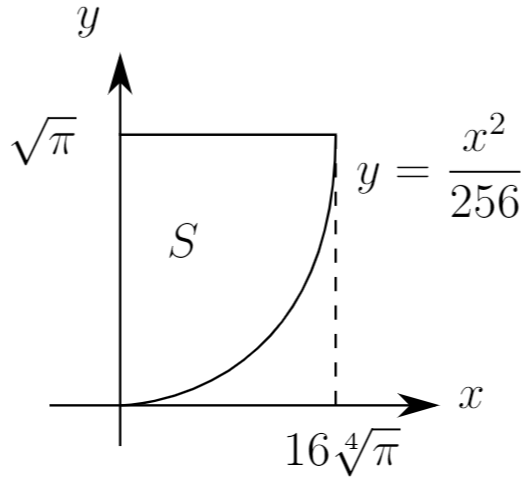
\includegraphics[scale=0.25]{drawing.png}
\end{center}

\noindent Чтобы поменять порядок интегрирования, нужно объявить $y$ независимой переменной. Из рисунка ясно, что $y$ меняется в пределах от $0$ до $\sqrt\pi$. Дуга параболы описывается уравнением $y = x^2/256$, а если выразить $x$, то получится $x = 16\sqrt{y}$ (отрицательную ветвь не берём, так как обе переменные принимают неотрицательные значения). Таким образом, переменная $x$ меняется в зависимости от переменной $y$ в пределах от $0$ до $16\sqrt{y}$. Переписываем интеграл (\ref{integral}) следующим образом и вычисляем:
\begin{equation*}
    I = \int\limits_0^{\sqrt{\pi}}\sin{y^2}\, dy \int\limits_{0}^{16\sqrt{y}} x\,dx = 128\int\limits_0^{\sqrt{\pi}}y\sin{y^2}\, dy = 64\int\limits_0^{\sqrt{\pi}} \sin{y^2}\,d(y^2) = -64\cos{y^2} \bigg|_0^{\sqrt{\pi}} = 128.
\end{equation*}

\end{document}